
%TODO Denne må skrives heil om: Sett av en dag til dette

%Eg forstår kvifor SANN ikkje har asynkron tid. For alle element må man kvar iterasjon gjennomføre lekkasje. Dette er brute-force måte å gjøre det på. Bedre er å bruke pow() eller løkker får den får innput gjennom synapse.
%Men det intuitive er å kjøre brute-force lekkasje kvar iterasjon. Bedre paralellisering om det gjøres alt på en gang. Gjør det slik, og skriv om kvifor!
%
%Hugs også at eg har laga arbeidskø av class tidsInterface, og alle som skal schedules er arvinger av denne. Dette gjør at det er mulig å simulere time-delay i synapse-overføring, axon-overføring, axon-hillock-AP-initiering, osv.





%*********************** SANN ***************************
%\chapter{Implementasjon: SANN}



%TODO Sjå design.tex (mot slutten er eit parti som er utkommentert som bestkrive s\_dendrite sin funksjon sammen med i_dendrite)





\section{SANN design and implementation}
\label{secSANN} 

	%TODO Lag plot:
	% 		- Figur som henger på veggen: auron-E-kretsen. (neural oscillator).
	% 		- Plott av lekkasje: Lekkasje kvart time-step v.s. å bare regne ut lekkasje kvart 30 tidssteg. ((skal være likt)).

% Frå section lekkasje:	%TODO Skriv i introen til section: om lekkasjen. Skriv om LIF. Internreferer!

% TODO Skriv mykje om lekkasje. Gjør dette avsnittet stort.

% SKRIV at dette er direkte simulering av neuronet i innledning.

%todo todo todo todo todo todo todo todo todo todo todo todo todo todo todo todo todo todo todo todo todo todo todo todo todo todo todo todo todo todo todo todo todo todo todo todo todo todo todo todo todo todo todo todo todo todo todo todo todo todo todo todo todo todo todo todo todo todo todo todo todo todo todo todo todo todo todo todo todo todo todo todo todo todo todo todo todo todo todo todo todo todo todo todo todo todo todo todo todo todo todo todo todo todo todo todo todo todo todo todo todo todo todo todo todo todo todo todo todo todo todo todo todo todo todo todo todo todo todo todo todo todo todo todo todo todo 

	SKRIV INNLEDNING TIL SANN.
	Her kan det være litt motivasjon, spiking-tid, og at det er lettest å lage dette ved direkte simulering av neuronet.
	Oppsummere litt det som er skrevet i ANN (sende litt bakover--referanser til ANN kapittel)

	SKRIV AT eg implementerer SANN for å bedre kunne sammenligne de to. Da kan eg sammenligne implementering også. (DO IT!)
	Vidare har eg då frie rammer til når sammenligninga starter. Testinga er ikkje basert på rammene til implementasjonen, men implementasjonen kan heller delvis være basert på rammene til test-case. Dette gir mykje friare testing.

	I innledninga: skriv det som står kommentert ut (tittelen). -at dette blir en simulering av mekanismene for enkeltneuron.

	Bør nok også skrive at alt dette er mitt arbeid, men har blitt gjordt før.
	Dette er ikkje eit argument for å gjøre arbeidet mitt større, men begrunne mangelen på 'cite'.
	Element i denne teksten kan likevel være nye, men siden eg ikkje har oversikt over tilstanden til SANN vil desse fremstega bli skrevet veldig mildt om dersom de skrives i det heile tatt.

	VIKTIG: få med problemer med SANN: forbered å lage eit "bedre" design for å løse desse problema! (Forbered skriving av kvifor eg starta å utvikle KANN, som skal skrives som innledning i \\section\{KANN\} \ref{secKANN}

	%\section{Simuating the mechanisms of the neuron}

	% Kjør masse sitering eller referering innad i dokumentet for å hente ut meir poeng fra sensor.
	% Skrive at "Alle SANN" istedenfor "the usual way ..". Det er litt vanskelig å skrive "alle" uten å være påståelig.
	% Ikkje skriv "usual way". Skriv heller at det er implementert som .. ( i dette prosjektet.. ). Skrive så at modellen SANN tilseier at dette er metoden..
	The usual way to implement spiking artificial neural networks (SANN) is a direct simulation of the mechanisms that generate the behaviour of the neuron.
	
	In terminology from graph teory, a neural netwoks is a directed cyclic graph with a dynamic amplification (weights) on its edges.
	The nodes of this graph are the neurons and the edges are the synapses between two neurons.% (The connection between them).

	In neural networks you have synaptic plasticity, or change of the weights of the edges. Synaptic plasticity is what is reffered to as learning in neuroscience. %TODO ref bear eller noke.


	Earlier ANNs can be said to be a set of nodes that transmits continous variables through its output synapses. The timing of such networks is synchrounous, and the transmission of each node is governed by a central clock.
	For networks of biologic neurons, the transmission is completely asynchronous, an the transmission happens whenever the neuron depolarization reaches the firing threshold.
	The value is increased or decreased by exitatory or inhibitory synaptic input, respectably .
	
	% Ny tanke: synaptisk plastisitet er kanskje større innerst på axonet: her er kanskje AP litt større, så når dette ganges inn med synaptisk effektivitet for å finne 'synaptic weight' vil dette gi at små endringer vil gi større utfall
	% 	for synapser som ligger tidlig på axonet. Dette er logisk dersom størrelsen på AP varierer.
	When the value of the node reaches the firing threshold for the neuron we get transmission through its output synapses.
	%When the value of the SN reaches the firing threshold, an action potantial is transmitted by letting the synapse add its weight to the postsynaptic neuron.
	As the action potential is seen as a boolean signal internally in the neuron, we get a constant depolarization on all the output synapses of a neuron.
	This depolarization gives the amount of neurotransmitter release. 
	Because this depolarization is constant over time, we can include this aspect into the synaptic weight of the edge, $W_{ij}$.
	In this simulation we simplify the transmission, and other effects of elements like pre--action potential depolarization of the synapse is not included.%XXX FORENKLA VEKK
	We then get that synaptic transmission can be executed by simply adding the synaptic weight to the postsynaptic neurons value.
	%SKrive at dette er vanlig, og at dersom det er ønskelig å innføre slike prinsipp, kan dette lett gjøres pga den modulære oppbygginga til simuleringa.
	The modular design of this implementation makes it possible to make changes to the indivitual elements without affecting the whole implementation.
	It is therefore not much work to implement elements such as short term plasticity and axo--axonic synapses in future uses of this simulator.
	% Forrige linja har kanskje ikkje så mykje med oppgava å gjøre?

	% Kanskje bare: "The neuron .."
	%The nodes of ANN are
	The neuron is
					 often modelled as a leaky--integrate--and--fire neuron (LIF-neuron). %TODO Referer.
	In this model the node ``leaks'' a certain amount of the potential, and the value decreases a over time. 
	% Skrive om ekvivalent kondensatorkrets?
	This value varies as a function of the value of the neuron, and we get a first order differential equation for the value of the node.
	For SANN nodes (SN) this is implemented as subtracting a product of the value every time iteration. 
	\begin{equation}
	v_t = v_{t-1} - v_{t-1}  \alpha % = (1-\alpha)  v_{t-1} Skal skrive egen section om dette. Sparer den siste godbiten..
	\end{equation}
	The leakage of value will be further discussed in section \ref{secTheLeakageForSANN}.

	Because every aspect that is thought important in neural signalling is simulated in SANN, 
		we can say that this is a direct simulation of each node of the network.   % KVA MEINER EG med direct manner? --At kvar ting er simulert kvart tidssteg. Naiv implementasjon. Ueffektivt!
	% Skriv kva eg meiner med "direct simulation". (at kvart elmement som er viktig simuleres for seg selv, kvart tidssteg. Nain implementasjon).
	%The simulation of the mechanisms of the nodes is 
	

	\subsection{The Nodes' Input}
	In this implementation, all transmissions through the input synapses arrive at the dendrite.
	Here the membrane potential is either increased or decreased, depending on whether the synapse is an exitatory og inhibitory synapse.

	Whenever the membrane potential goes to suprathreshold levels (value goes above the predefined firing threshold), an action potential is simulated.
	%When the membrane potential of the axon is higher than the firing threshold, specialized voltage gated channels are opened, and we get the self--carrying action potential. 
	As the biological acion potential initiates transmission in all the neuron's output synapses, the simulated action potential will initiate the ANN's version of a synaptic transmission.
	For a review of the biological action potential, it is referred to section \ref{ssecTheActionPotential}. %XXX Veit ikkje heilt korleis eg skal skrive : "gå tilbake til start (section ?? )".
	%Se section \ref{ssecTheActionPotential} for a description of the action potential in the biological neuron.
	
	% TODO Neste linja stater for svakt. Dersom det er debatert er det lite truleg. Framstill det som at dette ikkje er debattert (det er ikkje det. (?))
	%Another mechanism that is debated in the neuroscience community is the possibility of some intracellular signalling mechanism that will initiate the action potential.% at the axon hillock. %TODO referer!
	%This mechanism is initiated by a suprathreshold potentiation somewhere on the dendrite, sendt through the cytoplasm of the neuron to the axon hillock, where it will cause the initiation of an action potential.

	As synaptic input is defined to arrive at the dendrite in the emulated neuron, the dendrite is responsible for the action of recieving the transmission.
	This is done by the function \emph{s\_dendrite::newInputSignal(double)}.
	%As the function is inherited from \emph{i\_dendrite}, where it is defined as a pure virtual funtion, the function must be declared in class \emph{s\_dendrite}. XXX XXX XXX XXX Kjempeviktig poeng for "comparison"
	

	In the biological neuron, a new input signal changes the value of the postsynaptic neuron propotionally with the size of the transmission.
	The size of the transmission is given by the synaptic weigth $w_{ij}$.
	When a new transmission comes from a synapse, it is therefore the synaptic weigth that is sent into the postsynaptic dendrite.
	Because future use of the code may include short--term synaptic plasticity, or other aspects changing the size of the transmission from the synapse, the size of the transmission is sent in as an argument to the postsynaptic dendrite.
	% TODO Gjør setninga over lettare! =kortare!
	%As the size of transmission is given by the strength of the connection, the synaptic weight $w_{ij}$, the synaptic weight is what is sent in from the synapse.
	%Because of future use of the code may have short--term synaptic plasticity, the size of the transmission is sendt to the postsynaptic dendrite as an argument (se appendix \ref{appendixSynPlast} for a review of synaptic plasticity).



%UNDER: FEIL FOKUS, dette er ikkje biologi-kap.!
%	A dendritic input will change the electrical potential of the cytoplasm comparet to the extracellular fluid. This electrochemical potential will propagate with a small time delay through the cell body, to the axon hillock.
%	% Skriv at det også kan være andre time delays. Eg (og stavdahl) ser ikkje på strøm som treigt..
%	In this implementation, the time delay is implemented by having a small delay of one time iteration before initiating the action potential.
%	This is done by the mechanisms of the pWorkTaskQue (se section \ref{ssecTime} for more about pWorkTaskQue).% and section \ref{ssecSANNAP}).
%

	\subsection{The ``Leakage''}
	\label{secTheLeakageForSANN}
	%TODO Skriv i introen til section: om lekkasjen. Skriv om LIF. Internreferer!

	The LIF neuron is modelled as being leaky with respects to time. %TODO REFERER.
	One way of simulating leakage is to update the value every time iteration. %eller recalculate?
	The leak can be defined as a value propotional to last calculated value.
	As this is the value from the last time iteration, we get the equation for the new value $v_t$
	
	\begin{equation}
		v_t = v_{t-1} - \alpha v_{t-1} \; = (1-\alpha) \cdot v_{t-1}
		\label{eqOppdateringAvVerdiEtterLekkasjeSimpelVariant}
	\end{equation}

	As we are concerned with efficiancy in the simulation, recaluclating the value for each node every time iteration is not preferable.
	
	From eq. \eqref{eqOppdateringAvVerdiEtterLekkasjeSimpelVariant} it can be shown that 

	\begin{equation}
		v_t = v_{t-l} (1-\alpha)^{t-l}
		\label{eqLeakageForSANN}
	\end{equation}
	
	Where $l$ is the time iteration when the value was last updated.
	%Where $l$ is the last time iteration the value was updated.
	Because leakage is a diminishing mechanism for the value of the node, the value will not go above firing threshold as a consequence of leakage alone.
	This makes it safe to update the value only when the value is used.




%-----------------------------------
% Gammelt (er fortsatt der nede, kommentert ut..)
%	Where $n$ is the last time where the value was updated. 
%	Because leakage is a diminishing effect on the value, the value will not go above the firing threshold because of this effect alone.
%	This makes it entirely safe to use \eqref{eqLeakageForSANN} in the implementation of SANN.

----------------------------------------------------------------------------------------------\newpage




	%TODO TODO TODO TODO TODO TODO
%	For the discrete time system, the next iterations value is computed as the sum of the leakage and any new synaptic input signals.
%	%In the absence of input, 
%	Isolated from the input to the node, the updated value is given by the equation
%	\begin{equation}
%		v_t = v_{t-1} - \alpha v_{t-1} \; = v_{t-1} (1-\alpha)
%	\end{equation}

	For this implementation, the time design enables us to have an event based simulation of the neuron.
	This involves that the node is updated only when the value is changed.
	In this case we can make the calculation of leakage more effective by updating the value only when it is used.
	The equation for the effect of the leakage then becomes
% 	\begin{equation}
%		v_t = v_{t-n} (1-\alpha)^{t-n}
%		\label{eqLeakageForSANN}
%	\end{equation}
%	
%	Where $n$ is the last time where the value was updated. 
%	Because leakage is a diminishing effect on the value, the value will not go above the firing threshold because of this effect alone.
%	This makes it entirely safe to use \eqref{eqLeakageForSANN} in the implementation of SANN.

% todo? Her kan eg lage eit plott av auron1 som lekker kvar iterasjon og auron2 som venter 30 iterasjoner før den lekke. Desse vil ligge over kvarandre.
% Lag auron1-plott med .-plott og auron2 som @-plott. (sjå s_dendrite::calulateLeakage() : kommentaren seier at eg allerede har gjort forsøket. Funka fett.)

\begin{lstlisting}
inline void s_dendrite::calculateLeakage()
{ 
  // Calulates new value for the node
  pElementOfAuron->dAktivitetsVariabel *= 
    pow( (double)(1-ALPHA), (double)(time_class::getTid()-pElementOfAuron->ulTimestampLastInput) );
}
\end{lstlisting}



















	The leakage will be calculated every time the value of the node is used or changed.
	This means that whenever the dendrite gets a new transmission from one of its input synapses, \emph{s\_dendrite::calculateLeakage()} is called.

	\subsection{Action Potential in SANN}
	\label{ssecSANNAP}
	When the depolarisasjon of the membrane goes above the firing threshold, the s\_auron element of the node is inserted into pWorkTaskQue, causing a small timedelay before calling \emph{s\_auron::doTask()}.
	In this context, \emph{s\_auron} have the role of the axon hillock, and initiates the action potential by inserting a pointer to the node's s\_axon object into pWorkTaskQue.

	After the axon's time delay (depending on the number of serial axon segments), the axon segment's \emph{s\_axon::doTask()} is called, 
	%The next time iteration, the node's \emph{s\_axon::doTask()} will be called,
																			causing all the output synapses of the segment to be inserted into pWorkTaskQue.
	This time delay can be increased by having multible s\_axon elements in series, but for the initial testing of this simulator, one single axon segment was used to model the axon.
	In this case, the segment will contain all the node's output synapses.
	The time delay of the individual segments corresponds to the time it takes for the action potential to propagate through a segment of the biological system.
	Increased spatial resolution will almost have no affect the run--time efficiancy of the system. %TODO Test, eller argumenter! XXX
	%The time delay of the axon corresponds to the action potential propagating through the axon of the neuron in the biological system.

	Also the output synapses of the node will be executed by adding a pointer to the element to pWorkTaskQue.
	The delay here corresponds to the time delay of a synaptic transmission, due to the delay caused by the release of neurotransmittors(NT), diffusing of NT through the synaptic cleft and the activation of the postsynaptic receptors.
	% TODO Referer internt til BiologiskeSystemet.tex (Men først skriv om dette). Kanskje bedre å bare skrive om det der, og referere dit (skrive bare "corresponds to the delay of syn.transmission" (med ref. til bioSys) her..)
	After the time delay, the output synapse's \emph{s\_synapse::doTask()} will be executed, causing the excitation or inhibition of the postsynaptic node to each of the node's output synapse. 
	%, depending of the nature of each synapse (whether it is excitatory or inhibitory).
	
	The postsynaptic potential will change as a function of the synaptic weight. For this simulation the postsynaptic potential will change with a factor $\frac{1}{\alpha}$. %XXX Kvifor? 1/a. Sjekk regtek bok.
	This is handled in the postsynaptic dendrite, causing the postsynaptic depolarisasjon to change by $\pm \frac{W_{ij}}{\alpha}$, depending on the nature of the synapse.

	%TODO TODO OTOD TODO SKRIV OM dale's principle I BiologiskeSystemet.tex TODO TODO Og referer dit.
	In many ANNs the synapse has the ability to change between between being excitatory and inhibitory. 
	This corresponds to e.g. a positive synaptic weight becoming negative after synaptic plasticity.
	According to Dale's Principle %TODO \ref{REFERER RETT PLASS!}
		, in biology the synapses are either excitatory or inhibitory.
	%If the synaptic weight is zero the synapse dissapears.

	Synapses can not go from being excitatory to being inhibitory, and vice versa.
	In this simulation, excitatory and inhibitory synapses are therefore separated by a boolean \emph{bInhibitoryEffect}. The transmission is implemented in \emph{s\_synapse::doTask()} as
\begin{lstlisting}
inline void s_synapse::doTask()
{
  pPostNodeDendrite->newInputSignal( 
    (1-2*bInhibitoryEffect) * dSynapticWeight );
}
\end{lstlisting}
	When synaptic plasticity is implemented for this simulation, it is important to make shure that the synapse does not become negative. 
	The specific mechanisms of synaptic plasticity have not been designed, but when the synaptic weight comes to close to being zero, the biological synapse will dissapear.
	The plan is to make some condition for the dissapation of synapses as the synaptic weight becomes to small.
	%The spatial and temoral resolution can be improved by simply adding more input dendrites and axon elements for the node.
	%Each axon elements then gets the function of a segment of the ``axon proper'' in the biological neuron. %TODO Skriv kva "axon proper" er i BiologiskeSystemet.tex, og referer dit!

%TODO FLytt dette til resultat-kapittel. Kan referere dit, men bare med ei/eit par   setninger.
%XXX XXX XXX XXX XXX XXX XXX XXX XXX XXX XXX XXX XXX XXX XXX XXX XXX XXX XXX XXX XXX XXX XXX XXX XXX XXX XXX XXX XXX XXX XXX XXX XXX XXX XXX XXX XXX XXX XXX XXX 
\subsection{The response of the SN}
	In the previous sections, the design of each node for the SANN was introduced.
	The activity variable for the SN corresponds to the level of depolarization of the membrane potential for the biological neuron.
	Excitatofy synaptic input to a node will increase the value of the node and inhibitory synaptic input will decrease the node's value.

	%TODO Lag figur om kretsen. Den skal ligge her. Neste plott er resultatet, og kan komme på neste side, eller noke..
	\begin{figure}[hb!tp]
		\centering
		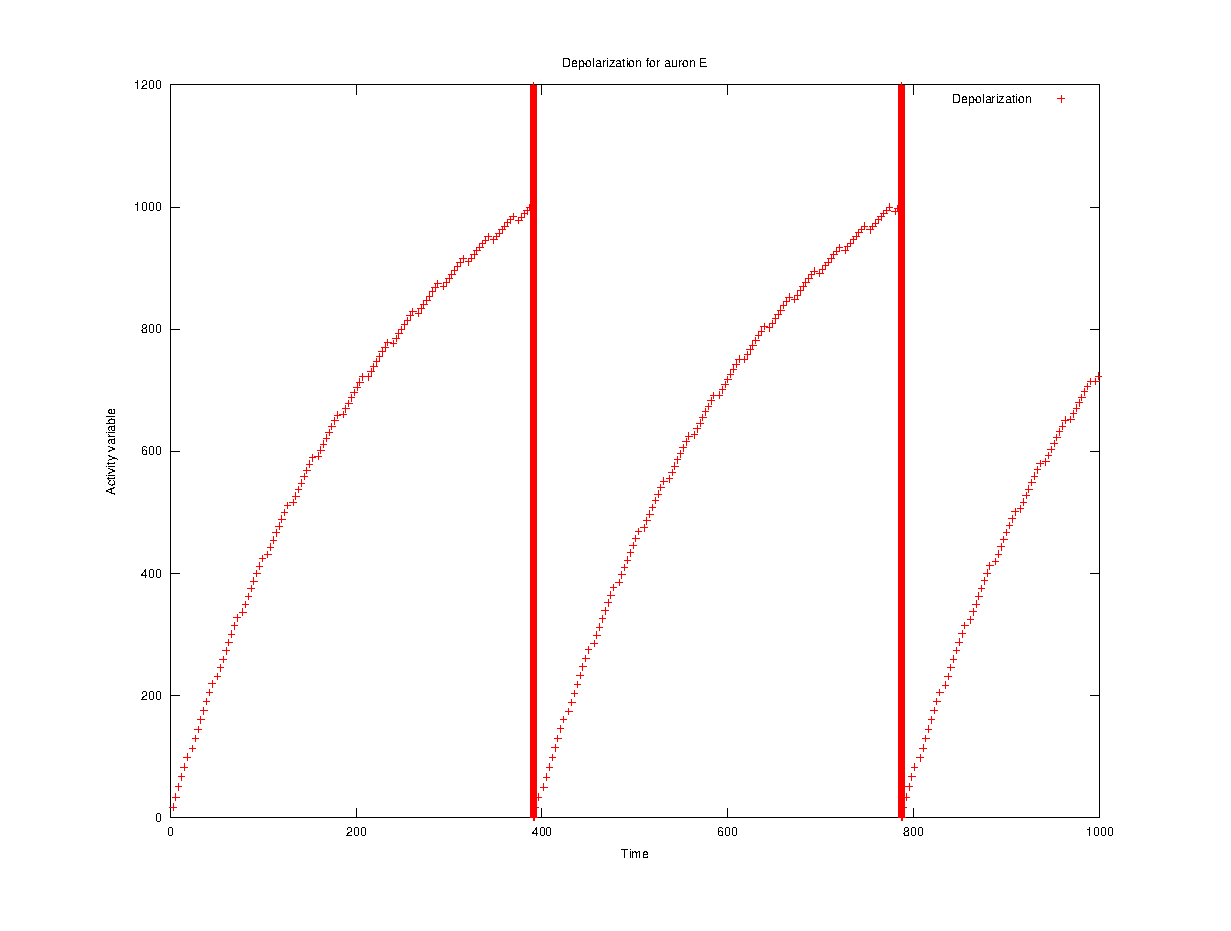
\includegraphics[width=0.95\textwidth]{depolPlotAvSN/eps_auronE-depol.eps}
		\caption{Depolarization plot for auronE in the neural circuit from fig ?. The activity variable for a SN corresponds to the depolarization of a neuron.} %TODO TODO Lag plot som beskriver kretsen, og referer dit, her.
		\label{figAuronE}
	\end{figure}

	Each time iteration, the value of the node will diminish due to ``leakage''. 
	In this implementation, the leakage is only computed whenever the value is used.
	This is done by the use of equation \eqref{eqLeakageForSANN}.

	%Skriv først (underveis i neste avsnitt) at for å teste dette kan vi lage en "neural oscillator", en krets som vil holdes aktiv av seg selv. Kvar output .. osv...
	To test the implementation of the SN, the circuit in fig. ? % XXX TODO Lag denne, og :  \ref{}
		was tested. The connections between node A1 and node A2 has a synaptic weight of weight $W_{21}=1$, large enough to excite node A2 above firing threshold in a single transmission.
	Each of the nodes A1-A9 has a synapse to the next node with a synaptic weight of one. 
	From node A9, there is a synapse to node A1 of weitht 1 completing the ``neural oscillator''. In this circuit each of the nodes will fire once every ninth time iteration.

	Except from node A7, every node in the ``neural oscillator'' have a synaptic connection to node E with a constant synaptic weight $W_{Ej}=0.017$ . %todo: ta vekk "constant" ?
	There is no synapse from A7 to node E.
	%From each of the nodes in the ``neural oscillator'' except for node A7, there is a synaptic connection to node E with a constant synaptic weight $W_{Ej}=0.0017$ .
	In the course of one period we therefore get eight excitatory inputs to node E, each transmission of size $W_{Ej}*\tau = 17$. Every ninth time iteration we get no input to node E.
						%period AV KA? Skriv kva!

	Fig. \ref{figAuronE} shows the resulting depolarization plot of node E. 
	We can se that node E gets a steady input from the nodes of the ``neural oscillator''.
	%
	Every cycle of the oscillator there is a pause in the excitatory input to node E, resulting in a small drop in node E's activity variable. 
	One cycle of the oscillator is represented by 8 entries in the log file, one log entry after each transmission.
	This can also be observed in fig. \ref{figAuronE} by remebering that during a pause in transmission, the change of value for the node is only due to the ``leakage'' of the node's value.
	Every 8'th value of node E's value is smaller than the previous entry due to this effect.
	%This is due to the absense of excitatory input and due to the leakage during the pause in excitatory input to the node.

	%After the pause in synaptic input to node E, the leakage is calculated at the time of the next transmission by eq. \eqref{eqLeakageForSANN}, resulting in the little drop in the node's value.

	% TODO flytt neste linja litt ned (eller noke, passer ikkje akkurat her..)
	Fig.\ref{figAuronE} is a direct result of the execution of the log files created by the simulator.
	% TODO Skriv det under i "log-file"-biden av design.tex! Passer ikkje her...
	%The constructor of every node creates a log file and each time the nodes activity variable is changed, the time iteration and the new value is written to the log file.
	%The destruction of each node finalize the node's log file, by writing octave calls that makes plots like the one in fig. \ref{figAuronE} and prints the resulting plot to an eps file.
	%Many of the eps files included in this report comes from the execution of similar octave script--file logs.

	We can also se that the mechanisms behind firing an action potential works. 
	%When the value of the node goes over the firing threshold an action potential is fired.  %XXX Dette er kanskje bedre måte å sei det enn neste?
	When the node's value goes to suprathreshold levels, an action potential is fired. %Skriv: dette er representert ved en vertikal strek i figuren (eller i logg-plottet).
	In fig. \ref{figAuronE} we can se that the node's value is reset to zero after firing an action potential.
	%TODO Ta med det neste, men ikkje før eg er heilt sikker, og kan gjøre det til meir enn en påstand (ta med noke i appendix, eller skrive tidspunkt for de to)
	%In the corresponding log file for the synaptic transmission of node E's output synapses, it can be observed that the synaptic transmission comes two time iterations after the node's value reaches the firing threshold. 
	%%Similar plots of the synaptic transmission from the synapses log file shows transmission after the time delay caused by the initiation of an action potential and the delay caused by the action potential propagating through the axon.
	%TODO Være sikker på at det er har skrevet her er heilt rett. (flaut dersom det er en åpenbar feil, her!)
	Analysis of the log files shows that node E fires one action potential at time 391 and one at time 787.
	The synapse's log file shows transmission at time 393 and 789, each at two time steps after node E's value goes above firing threshold.
	%each transmission at two time iterations after node E's value goes above the firing threshold. 
	This tells us that the simulated delay caused by the action potential initiation and propagation works as designed.
	% Auron E: AP    på tid: 391 og 787
	% Syn overføring på tid: 393 og 789
	
	The log entry for the next time iteration is zero, due to the simulated refraction period of the node.
	Two time iterations after the action potential the node's value becomes or 17. %TODO? Skal eg skrive litt om at eg kjører størrelse på W_ij i kor mykje postsyn. går mot fyring. I promille? Viktig poeng!
	%Har sjekka: Dette gjelder for begge overføringene/AP i simuleringen. Skriv dette, og at det betyr at vi for desse to overføingene faller "pause" ikkje til to tidssteg etter fyring.
	This corresponds to the defined synaptic transmission for each of the synpses of the circuit. %Kanskje heller : ".. for the synapse in question"? ELLER at dette betyr at i desse tilfellene har vi ikkje pause på dette tidspunktet.

	%This analysis shows that the above discussed design of the simulated neuron gives us the mechanisms of the neuron, in respect to synaptic transmission, leakage, refraction time and action potential firing.
	This analysis shows that, in respect to synaptic transmission, synaptic leaky integration, refraction time and action potential firing, the design and implementation gives the behaviour of the model used. 
																																														  %ELLER: .. considered model of the neuron.
	%TODO Skriv om den siste linja litt. (siste bit: kanskje heller: "... , the design and implementation gives the desired behaviour for the simulated neuron."?




%	\subsection{Analysis of the SN's value curve}
	% TODO TODO TODO TODO TODO TODO TODO TODO TODO TODO TODO TODO TODO TODO TODO TODO TODO TODO TODO TODO TODO TODO TODO TODO TODO TODO TODO TODO TODO TODO TODO TODO TODO TODO 
	% Gjennomfør ei analyse av kurva. (Meir enn/istedenfor den siste linja over).
	% TODO TODO TODO TODO TODO TODO
	%We can se that the value of the node has a vaulue % at det varierer som plot X (finn eit plott, legg det inn i BiologiskeSystemet.tex, referer dit, her) %TODO
%	Fig. \ref{figAuronE} resemples a plot of a step responce of a condencator, with an extra non--linearity when the value of the node crosses the firing threshold.
%	We have already analyzed the 
%	Skriv at kurva ser rett ut.





	



% Feil ved denne forenklinga:
%  - vi går ut fra at verdien ikkje lekker mellom dendrite og axon hillock. Dette er nok litt feil, men ikkje mykje.
% 	Dersom vi hadde hatt dette, måtte vi implementert lekkasjen, men også en liten time delay før verdien blir lagt til verdien i axon hillock. Dette er computationally ineffektivt.
% 	Dersom dette skal implementeres (at programmet skal være en simulering av neurale system, så er dette mulig ved å ha en egen node for axon hillock)
	
	
	%TODO Skriv korleis dette kan gjøres for KN.

	% Lag diagram om korleis dette funker. Kanskje eit "uml-signal diagram"?   (Treng fleire figurer her!)

	% TODO Lag en figur som viser oppsettet til kretsen.



%TODO TODO Lag eit plott som sammenligner kontinuerlig lekkasje, vs beregning av lekkasje etter 30 iterastions. (Dette skal inn her..)






% (Neste som kommer er KANN--implemenasjon-kapittelet)
